%% \section*{Making an {\it ATLAS} of $z\approx6$ Quasars with the {\it James Webb Space Telescope}}


%%
%% ENTER TEXT AND FIGURES BELOW
%%
\noindent
{\it As the Chandra X-ray Observatory looks towards its 20th year of
operation, its scientific legacy is secure and includes a deeper
understanding of the physics of black holes, accretion and AGN.  We
propose to build on this legacy in the area of the highest redshift
quasars $z > 6$, which will not be accessible again until the
Lynx/Athena era in the 2030s. We aim to observe four recently
discovered $z > 6$ quasars, which have high luminosities and massive
black holes ($M_{BH}\approx1-6\times10^9M_\odot$). All 4 quasars have
been detected in ALMA $850\mu$m imaging. We shall: measure the full
photon budget of luminous $z > 6$ quasars; correlate the strength of
Lyman-$\alpha$ and X-ray absorption; look for quasar X-ray
variability; and study the link between the accretion disc and coronal
emission in quasars. This final science aim will allow the extension
of the Quasar Hubble diagram to $z > 6$, significantly further than the
$z<1.2$ extent of the Type Ia SNe Hubble diagram.}

\smallskip
\smallskip
\noindent
{\bf Introduction:} Very high redshift quasars with $z\gtrsim6$ are
excellent probes of the early Universe. This includes studies of the
Epoch of Reionization for hydrogen (see Fan et al. 2006 and Mortlock
2016 for reviews) the formation and build-up of supermassive black
holes (e.g., Rees 1984, Wyithe \& Loeb 2003, Volonteri 2010, Agarwal et
al. 2016, Valiante et al. 2018, Latif et al. 2018) and early metal
enrichment (e.g., Simcoe et al. 2012, Chen et al. 2017, Bosman et
al. 2017). Indeed the search for $z\gtrsim6$ quasars has been a large
motivation for new optical and infrared wide-field surveys, and
projects including PanSTARRS, DES, VST ATLAS, UKIDSS, VHS and WISE
have led to a large increase in the number of $z\gtrsim6$ QSOs
identified (e.g., Willott et al. 2010; Venemans et al. 2013; Matsuoka
et al. 2016; Ba\~{n}ados et al. 2016; Tang et al. 2017; Yang et
al. 2017, Ba\~{n}ados et al. 2018)

\smallskip
\smallskip
\noindent
Recenlty, our team (Carnall et al. 2015; Chehade et al. 2018) reported
the discovery of four bright high-redshift quasars using the
combination of the VST ATLAS and WISE surveys (see
Figure~\ref{fig:xshooter} and Table 1).  Preliminary virial mass
estimates based on the \civ and \mgii emission lines give supermassive
black hole (SMBH) masses in the range $M_{\rm BH} \approx 1 - 6\times
10^{9} M_{\odot}$ for the four ATLAS quasars.  As such, Chehade
et~al. (2018) claim, along with Wu et al. (2015) that $\sim$0.1-0.6
and $\sim$1.2$\times 10^{10}$ M$_{\odot}$ SMBHs exist at $z\approx6.0$
and $z\approx6.3$, respectively. {\it These are the most luminous
quasars, with the most massive black holes at any redshift.}


\smallskip
\smallskip
\noindent
Chehade et al. (2018) claim, along with e.g Wu et al. (2015, Nature,
518, 512) that $\sim$0.1-0.6 and $\sim$1.2$\times 10^{10}$ M$_{\odot}$
exist at $z\approx6.0$ and $z\approx6.3$, respectively. These are the
most luminous quasars, with the most massive black holes, at any
redshift.

\smallskip
\smallskip
\noindent
``Understanding First Light \& Reionization'', that is, aiming to
understand the $z \gtrsim 6$ galaxy and quasar population is a key
science goal of {\it JWST}.

\smallskip
\smallskip
\noindent
We propose to obtain NIRSpec Long Slit
data on four $z\gtrsim 6$ luminous quasars that were identified
cleanly by their optical-to-WISE colours (the only such selection in
the literature). With these data, plus our we will be able to:
\begin{itemize}
\item Characterise the full rest UV-optical spectrum of the
$z\gtrsim6$ quasar population, from blueward of \lya to redward of
H-$\alpha$ ($\approx 1160 - 7330 \angstrom$ rest);
\item measure to 0.3dex (TBC!) the mass of the supermassive black
hole;
\item infer continuum shape, including measuring the contiuum slope at
both shorter and longer than $\lambda_{\rm rest} = 4000 \angstrom$;
\item infer the metalicity of the immediate environment of the quasar;
\item by linking to the GTO High-$z$ quasar programs, extend the
baseline and challenge BH-formation models; how do you have $\sim
6\times$10$^9$ $M_{\rm BH}$ in place $\lesssim$1.2 Gyrs after the Big
Bang?
\end{itemize}


%\smallskip
%\smallskip
%\noindent
%{\bf General Idea::} \\
%NIRSpec spectroscopy (Long Slit? IFU?) of the 4 ATLAS-WISE $z \approx 6$ quasars.\\
%\begin{itemize}
%\item BH masses
%\end{itemize}



\smallskip
\smallskip
\noindent
Questions to answer/things to address:: 
\begin{itemize}
\item Why not {\it HST}??
  \item Why not {\it ALMA}?? Have ALMA data...
\end{itemize}


\hspace{-7.5cm}
\begin{figure}[h]
  \begin{center}
    \hspace{-0.5cm}
%    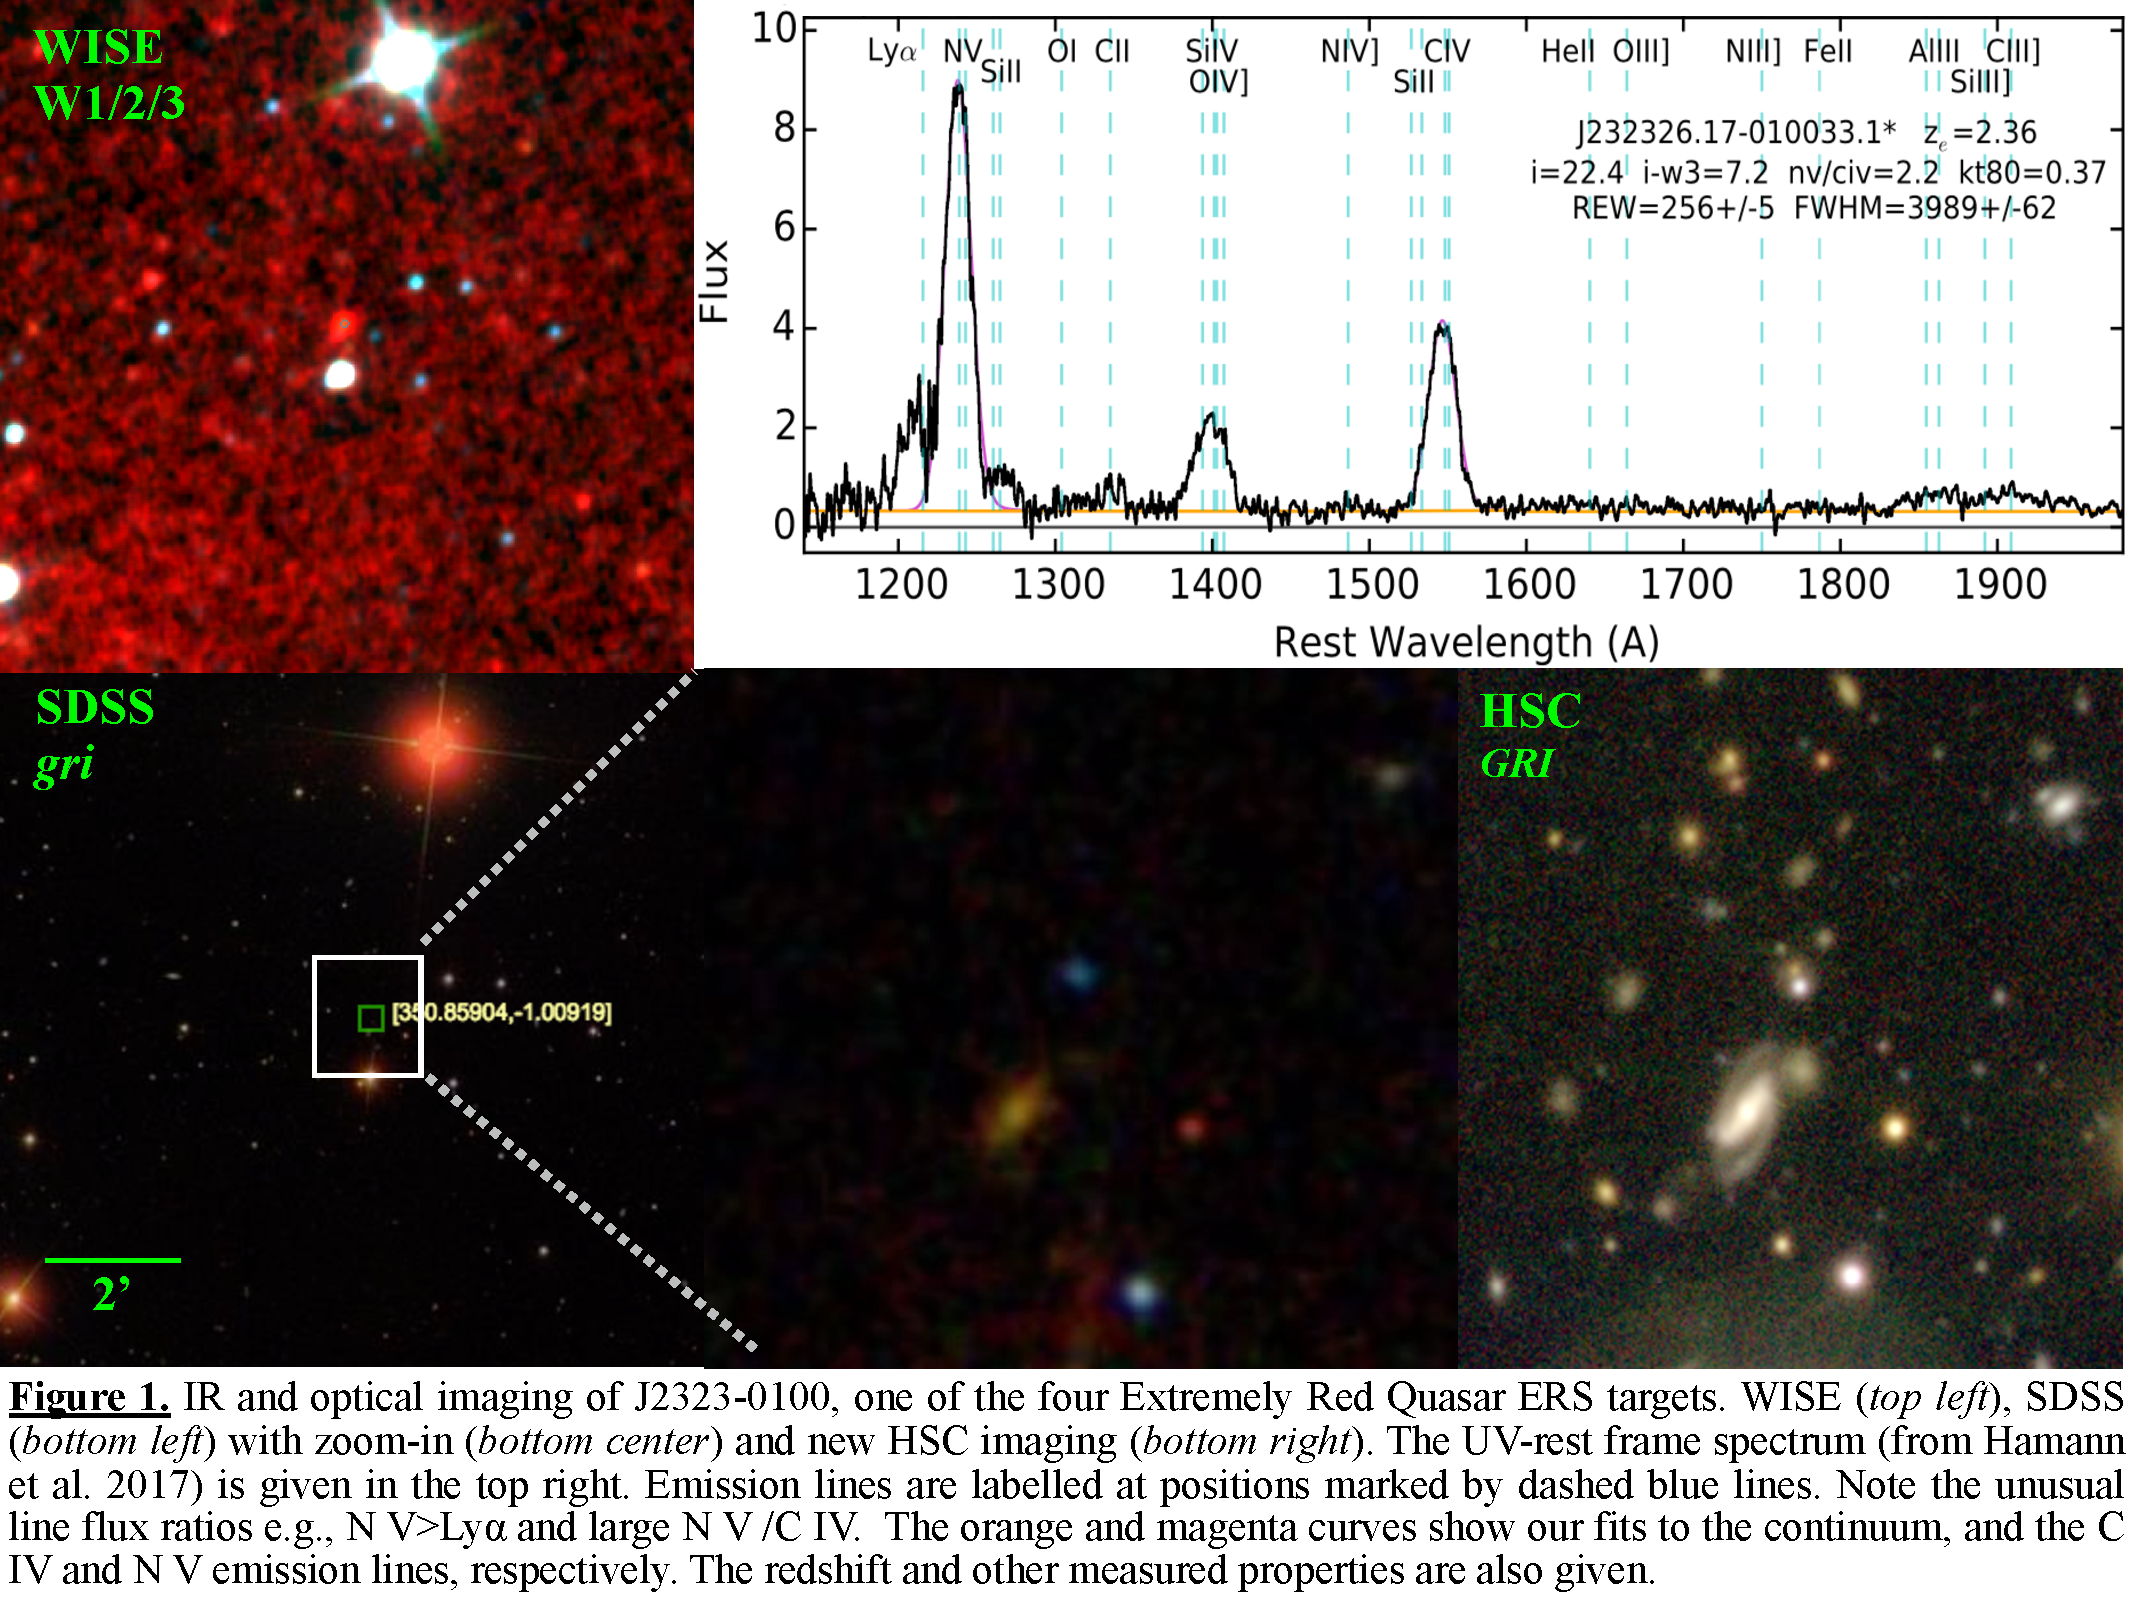
\includegraphics[]{WISE_SDSSzoomHSC_ERQ-image_v2.pdf}
    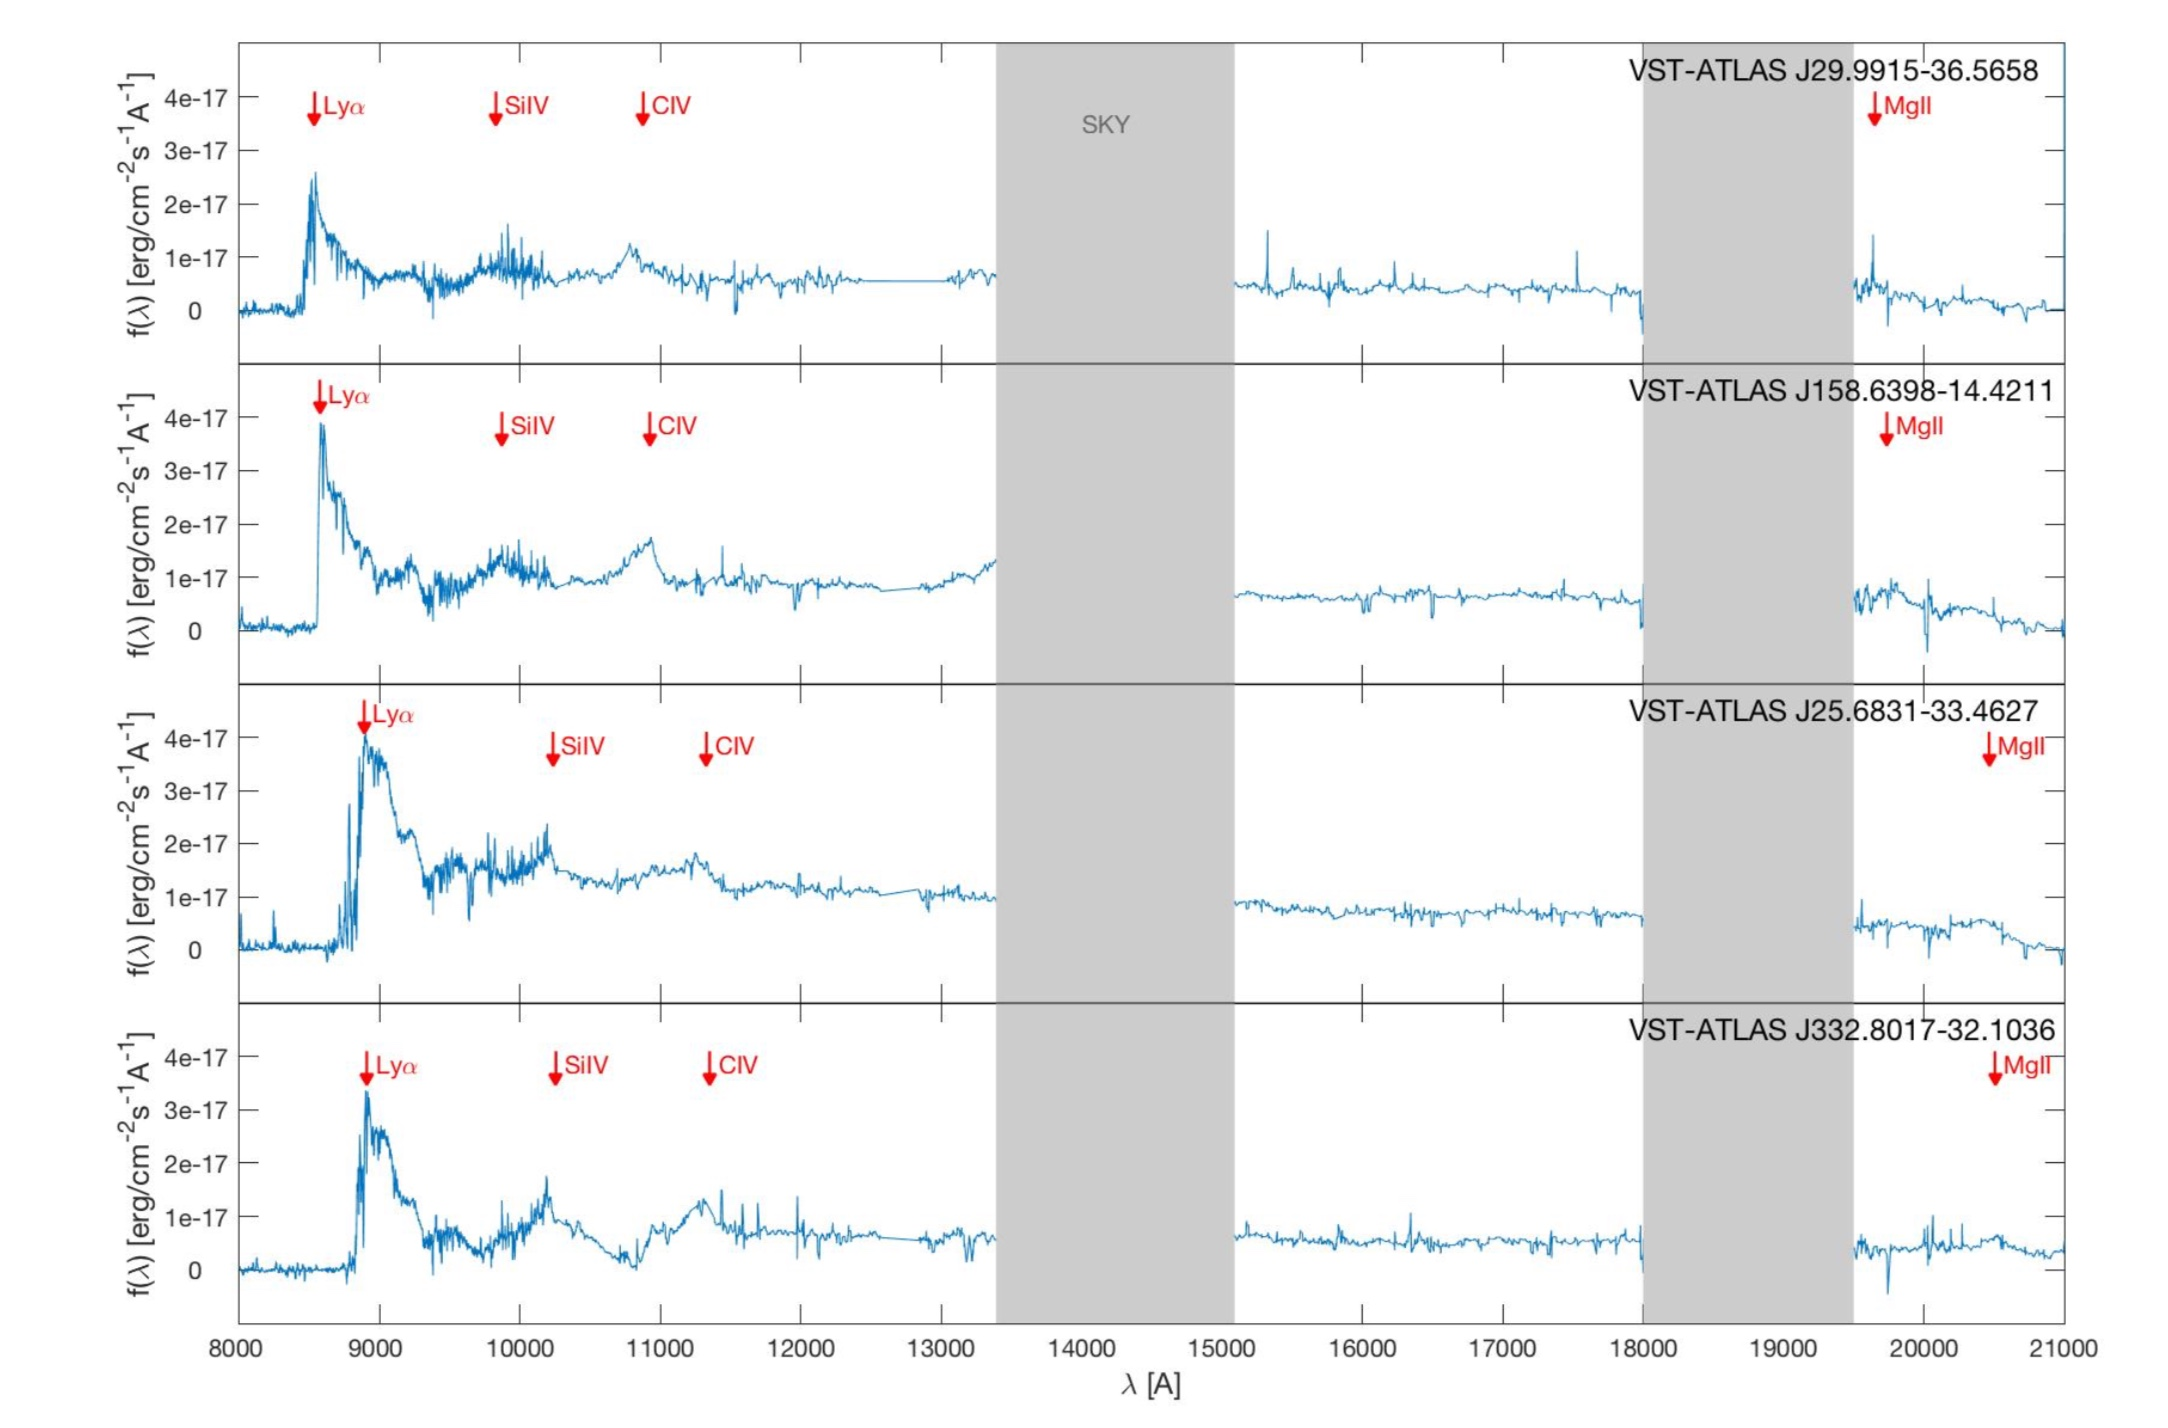
\includegraphics[height=12.0cm,width=16.0cm]{XShooter_spectra_Chehade2018_Fig2.jpeg}
    \vspace{-10pt}
    \caption{\footnotesize  
      The VLT X-shooter spectra for our 4 ATLAS quasars. 
      The spectra
      were flux calibrated to the observed $z$-band magnitudes from VST ATLAS
      and corrected for telluric absorption. 
      The positions of the Ly$\alpha$, Si IV, C IV and MgII 
      emission lines are marked (and the redshifts given in Chehade et al. 2018). 
      We note that higher ionisation lines such as C IV
      are frequently found to be blueshifted with respect to lower ionisation
      lines like Ly$\alpha$ and this is seen to be the case for all four
      quasars.}
    \label{figtest-fig}
  \end{center}
\end{figure}

\smallskip
\smallskip
\noindent
{\bf General Sample::} \\

\begin{table*}
\begin{center}
\begin{tabular}{ccccc}
\hline
 Quasar            & Redshift  & $z$ (AB mag)     & $M_{1450 \angstrom} $ &  Reference\\
\hline
 ATLAS J025.6821-33.4627 & 6.31 $\pm$  0.03 & 19.63 $\pm$ 0.06 &  -27.50 $\pm$ 0.06& \cite{Carnall2015}\\
 ATLAS J029.9915-36.5658 & 6.02 $\pm$  0.03 & 19.54 $\pm$ 0.08 &  -26.97 $\pm$ 0.08& \cite{Carnall2015}\\
 VIKINGKiDS J0328-3253   & 5.86 $\pm$  0.03 & 19.75 $\pm$ 0.12 &  -26.60 $\pm$ 0.04& \cite{Venemans2015b}\\
 ATLAS J332.8017-32.1036 & 6.32 $\pm$  0.03 & 19.75 $\pm$ 0.06 &  -26.79 $\pm$ 0.06& This paper \\
 ATLAS J158.6938-14.4211 & 6.07 $\pm$  0.03 & 19.44 $\pm$ 0.08 &  -27.23 $\pm$ 0.08& This paper \\
 PSO J340.2041-18.6621   & 5.98 $\pm$  0.03 & 19.67 $\pm$ 0.10 &  -26.42 $\pm$ 0.10& \cite{Banados2014}\\
\hline
\end{tabular}
\end{center}
\caption{Absolute magnitudes for the  four quasars discovered and the two quasars rediscovered 
in VST ATLAS+WISE. The ATLAS quasar absolute magnitudes are estimated via the X-Shooter spectra in Fig. \ref{fig:xshooter}
and the other two from the above sources.}
\label{table:absmag}
\end{table*}

\smallskip
\smallskip
\noindent
We propose to obtain ...sec exposures from {\it JWST} NIRSpec on each
of these four ATLAS $z>6$ quasars, for a total of sec.  With these
observations, plus our current multiwavelength data, our main science
goals are:
\begin{itemize}
\item Challenge SMBH formation models; how do you have $\sim$$6-10
  \times 10^{9}$ $M_{\odot}$ SMBHs in place $\lesssim$0.9~Gyrs after the
  Big Bang?
\item Measure the full photon budget of luminous $z>6$ quasars
  putting strict limits on the Eddington limit and radiative efficiency;
\item Check for variability (as is expected for super-Eddington accretion);
\item Link the gas content of $z>6$ quasar hosts via Ly-$\alpha$,
  dust emission and X-ray absorption;
%\item Double the number of  $z>6$ quasars with $>$40 net counts in the 0.5-7.0 keV energy range. 
\end{itemize}
%Our ancillary science aims include: complementing the {\it JWST} $z>6$ quasar GTO programs, as well as our own upcoming {\it JWST} GO Cycle 1 program, and cementing {\it Chandra}'s legacy of the very high-$z$ Universe.


\smallskip
\smallskip
\noindent
{\bfseries \textsc{Science Case}}

\smallskip
\smallskip
\noindent
{\bf The full photon budget of luminous $z>6$ quasars.} 
These $z>6$ ATLAS quasars are amongst the brightest quasars with the
most massive black holes seen at any redshift and yet appear less than
1~Gyr after the Big Bang.  The paradox is that in their rest optical
spectra they look very similar in e.g. metallicity to their lower
redshift counterparts. The $M_{BH}$ of these 4 quasars are close to
the theoretical maximum black hole mass achievable by luminous
accretion ($\approx10^{10}M_\odot$, see Natarajan \& Treister 2009,
King 2016; Gallerani et al. 2017), and the challenge is to understand
how these SMBHs have formed in less than $\approx$1~Gyr. This has led
to various speculations about how to seed black holes: either the
seeds have to be small and grow fast, or, they have to start big and
grow at a normal rate. The former scenario could mean that the
proto-quasars have frequently to accrete at super-Eddington rates to
speed their growth. The latter scenario suggests that to explain the
existence of SMBHs at high redshift, might include the possibility of
direct collapse black holes (DCBHs) where gas collapses without
fragmenting into stars to form an $\approx$10$^5 M_{\odot}$ black hole
seed. This has led to searches for these proto-quasars in
multi-wavelength surveys including X-rays.

\smallskip
\smallskip
\noindent
Here we are proposing to measure X-ray fluxes for 4 quasars whose
black hole mass is most difficult to explain and that we are seeing
shortly after their seeding phase. Clearly determining the full photon
budget at all wavelengths is vital in establishing their origin and
the nature of their host galaxies. Because of their high luminosity,
already these are some of the best studied quasars with optical and
NIR spectroscopy available from VLT XShooter, and ALMA observations of
the dust continuum and [CII] emission of the host galaxies. {\it Adding
X-ray luminosities to their multi-wavelength spectra will directly help infer
how such large mass objects appeared in the early Universe 
(e.g.  Valiante et al., 2018a; Valiante et al 2018b).} 





\smallskip
\smallskip
\noindent
{\bf Variability of luminous high-$z$ Quasars}. 
We have now entered the ``time-domain'' astronomy era, where we now
have large samples of variable quasars (e.g. SDSS-IV: TDSS with 100,000 objects).
Considering the rapid build-up of BH mass, luminous $z>6$ quasars
might have some of the largest $\dot{M}$ changes.  However, we have not
conclusively observed this.

\smallskip
\smallskip
\noindent
Nanni et al. (2018) report on the $z = 6.31$ quasar SDSS
J1030+0524. They note that when compared with data obtained by
XMM-{\it Newton} in 2003, the {\it Chandra} observations in 2017 show
a harder ($\Delta \Gamma \approx -0.6)$ spectrum and $\times$2.5
fainter flux. Although this is consistent with accretion disc state
changes i.e.  faint-hard, bright-soft, {\it the timespan of $\sim$2
yrs rest-frame, is unexpected for such a luminous quasar powered by a} 
$>$$10^{9} M_{\odot}$ SMBH. Nanni et al (2017) note that ATLAS
J025.6821-33.462 has a survey observation in 2007 by the NASA {\it
Swift} XRT and $\sim$3$\sigma$ detections in the 0.5-7, 0.5-2 and
2-7keV bands.  Thus making a measurement again, e.g. $\sim$2 years
later in the rest-frame, is now timely. Very high-$z$ quasars
potentially build-up their mass via super-Eddington accretion; if so,
we should observe these objects to be variable.

\vspace{-28pt}
\noindent
{\bf The gas content of $z>6$ quasar hosts via LyA, dust emission and
X-ray absorption:} All 4 ATLAS quasars are strong ALMA $850\mu$m
continuum sources at the $\approx0.5$mJy level
(Figure~\ref{fig:alma}). The detection of X-ray emission by {\it
Swift} XRT of J025-33 clearly shows that $z>6$ quasars can be strong
X-ray (and UV) emitters while being hosted by a dusty star-forming
galaxy. Indeed $z>6$ quasars seem characterised by strong dust and
$[CII]$ emission. (see e.g. Decarli et al 2018). Given this prevalence
of dust emission and $[CII]$ in high redshift quasars it seems natural
to search for absorbed X-ray emission to test for the presence of
neutral gas. In lower redshift quasars there has also been some
evidence seen for the presence of sub-mm emission from X-ray absorbed
quasars (e.g., Lutz et al 2010; Hill \& Shanks 2011; Bielby et al
2012; Heywood et al 2013) further motivating this search for X-ray
absorption at $z>6$.


%%\Huge \huge \LARGE \Large \large \normalsize (default) \small \footnotesize \scriptsize \tiny
\hspace{-7.5cm}
\vspace{-14pt}
\begin{figure}[h]
  \begin{center}
    \hspace{-0.5cm}
    \includegraphics[width=\textwidth]{Figures/j332_alma_lyA.png}
    \vspace{-10pt}
    \caption{\footnotesize
     {\it Left:} ALMA 850 micron dust continuum images for J332 showing an
      integrated flux density of $\approx0.5$mJy. The lower of the two ALMA sources is the quasar. The other 
      source could also be associated with the quasar. 
{\it Right:} Also the XShooter spectra of
      Chehade et al (2018) showing the complicated neutral gas pattern around
      this quasar via the Lyman-$\alpha$ absorption lines. Fig. 3 of Chehade et
      al shows the wide variety of Lyman-$\alpha$ absorption around the 4 ATLAS
      quasars. We propose to test for correlations between the presence of
      X-ray absorption, the pattern  of the Lyman-$\alpha$ absorption and
      the strength of dust emission.}
\vspace{-14pt}
\label{fig:alma}
  \end{center}
\end{figure}
\normalsize


\smallskip
\smallskip
\noindent
{\bfseries  \textsc{Why James Webb?}}
{\bfseries  \textsc{Why Now?}}


\vspace{-34pt}
\section*{References}
%%\Huge \huge \LARGE \Large \large \normalsize (default) \small \footnotesize \scriptsize \tiny
\footnotesize
Agarwal et al., 2016, MNRAS, 459, 4209 $\bullet$ 
Ba\~{n}ados et al., 2016, ApJS, 227, 11 $\bullet$
Ba\~{n}ados et al., 2018, Nature, 553, 473 $\bullet$ 
Bielby et al 2012, MNRAS, 419, 1315 $\bullet$ 
Bisogni, Risaliti, \& Lusso, 2017, arXiv1712.07515v1 $\bullet$ 
Bosman et al., 2017, MNRAS, 470, 1919$\bullet$
Carnall et al., 2015, MNRAS, 451, L16 $\bullet$ 
Chehade et al., 2018, MNRAS accepted, arXiv:1803.01424v1  $\bullet$ 
Chen et al., 2017, ApJ, 850, 188 $\bullet$
Fan, Carilli \& Keating, 2006, ARA\&A, 44, 415 $\bullet$
Giallongo et al., 2015, A\&A, 578, A83 $\bullet$ 
Heywood et al 2013, MNRAS,428, 935  $\bullet$ 
Hill \& Shanks 2011, MNRAS, 410, 76  $\bullet$ 
Latif et al., 2018,   arXiv:1801.07685v1 $\bullet$
Lusso et al., 2010 , A\&A, 512, A34 $\bullet$
Lusso \& Risaliti, 2016, ApJ, 819, 154	$\bullet$
Lusso \& Risaliti, 2017, A\&A, 602, A79	$\bullet$
Lusso \& Risaliti, 2017, arXiv1712.09656v1	$\bullet$
Lutz et al 2010, ApJ, 712, 1287 $\bullet$
Matsuoka et al., 2016,  ApJ, 828, 26 $\bullet$ 
Nanni et al., 2018, arXiv:1802.05613v1  $\bullet$ 
Nanni et al., 2017, A\&A, .603, A128	$\bullet$ 
Mortlock et al., 2011, Nature, 474, 616 $\bullet$ 
Mortlock, 2016, in {\it Understanding the Epoch of Cosmic Reionization: Challenges and Progress}, 423, 187 $\bullet$
Rees, 1984 ARA\&A, 22, 471 $\bullet$
Risaliti \& Lusso, 2015, ApJ, 815, 33 $\bullet$ 
Risaliti \& Lusso, 2017, AN, 338, 329 $\bullet$
Simcoe et al., 2012, Nature, 492, 79$\bullet$
Steffen et al., 2006, AJ, 131, 2826 $\bullet$
Tang et al., 2017, MNRAS, 466, 4568 $\bullet$ 
Valiante et al., 2018a, MNRAS, 474, 3825$\bullet$
Valiante et al., 2018b, MNRAS, 476, 407 $\bullet$
Vanden Berk et al., 2001, AJ, 122, 549 $\bullet$
Venemans et al., 2013, ApJ, 779, 24 $\bullet$  
Volonteri, 2010, A\&ARv, 18, 279$\bullet$
Wu et al., 2015, Nature, 518, 512 $\bullet$
Willott et al., 2009, AJ, 137, 3541 $\bullet$
Willott et al., 2010, AJ, 139, 906 $\bullet$
Wyithe \& Loeb, 2003,  ApJ, 586, 693 

%(eg 



%%%%%%%%%%%%%%%%%%%%%%%%%%%
%%%%% End of document %%%%%
%%%%%%%%%%%%%%%%%%%%%%%%%%%

%\end{document}

